%TC:ignore

\newpage 
\section*{Typesetting Conventions}
\begingroup
\footnotesize 

\subsubsection*{Text formatting}
Template instructional text is typeset as follows in a sans-serif font, for example:

\instr{
Provide information on the preparation and delivery of this application by the department.
This should include:
\begin{itemize}
\item a description of the self-assessment team, including comment on the roles and
responsibilities of individuals, and how these were assigned. 
\end{itemize}
}

Regular text is typeset in a serif font.

\subsubsection*{Figures and Tables}
All tables and figures are identified by three-part numbers: the first two parts indicate the section; the third part is a counter within that section. For example, Table 2.1.15 would be the 15\textsuperscript{th} table within Section~2.1.
Some tables are zero-inflated; to maintain readability of those tables, zeros are replaced with dashes, for example:

\begin{tabbox}{!ht}
\footnotesize 
\sffamily \\[1mm]
\textbf{Example Table} Example table with many zeros, replaced by dashes\\
    
\begin{tabular}{p{3cm}
                C{1cm}
                C{1cm}
                c
                p{0.5cm}
                C{1cm}
                C{1cm}
                c
                !{\qquad}
                C{1cm}}
\toprule 
  & \multicolumn{3}{c}{Permanent/CID} && \multicolumn{3}{c}{Fixed-Term}\\
  \cmidrule{2-4}\cmidrule{6-8}
  Grade & {M} & {F} & \%F && {M} & {F} & \%F & Total\\
  \midrule 
  Academics \\
  \midrule   
  Professor& 4& -& -&&- &- &- & 4\\
  \hdashline   
  Professor (Scale 2) &4 & -&- &&- &- &- &4\\
  \hdashline   
  Senior Lecturer &5& -&- &&- &- &- & 5\\
  \hdashline   
  Lecturer (above bar)&14 &1 &6.7\% &&1 & -&- & 16\\
  \hdashline   
  Lecturer (below bar)&- &1& 100\% && 2&1 & 33\% & 4\\ 
\bottomrule 
\end{tabular}

\end{tabbox}

This document contains many figures presenting Likert-scale responses; in cases where the numbers do not fit well, these are filtered out, as in the example figure below. 
\begin{figbox}{!ht}
\footnotesize 
\sffamily \\[1mm]
\textbf{Example Figure} Likert-scale response with filtered numbers\\
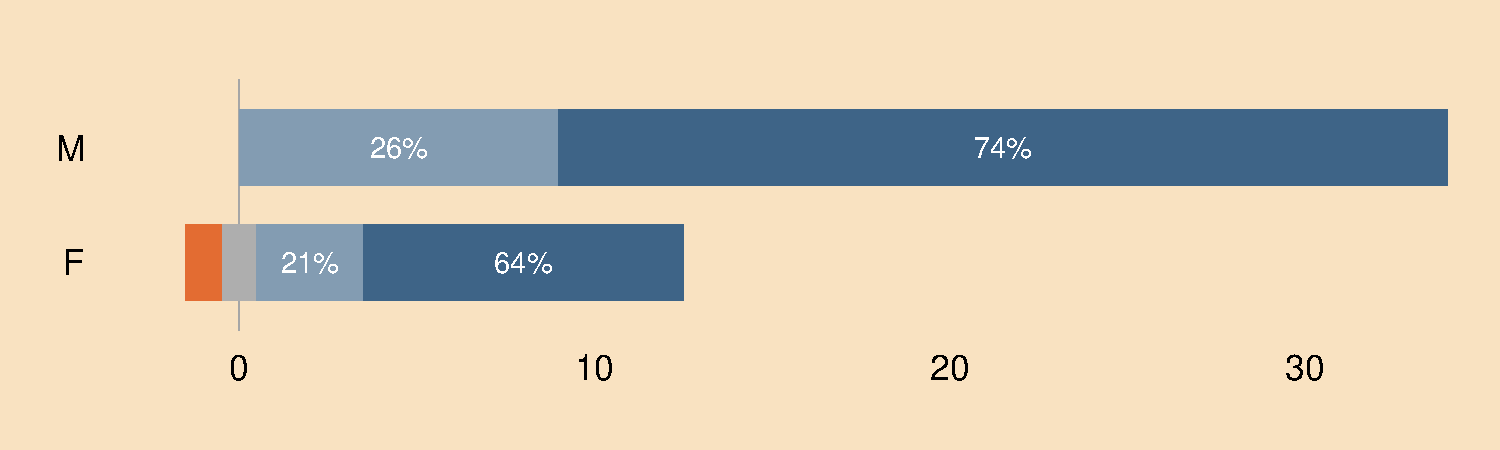
\includegraphics[align=t,trim={0 5mm 0 15mm},clip,width=10cm]{fig/culture/paolo8.pdf}\\
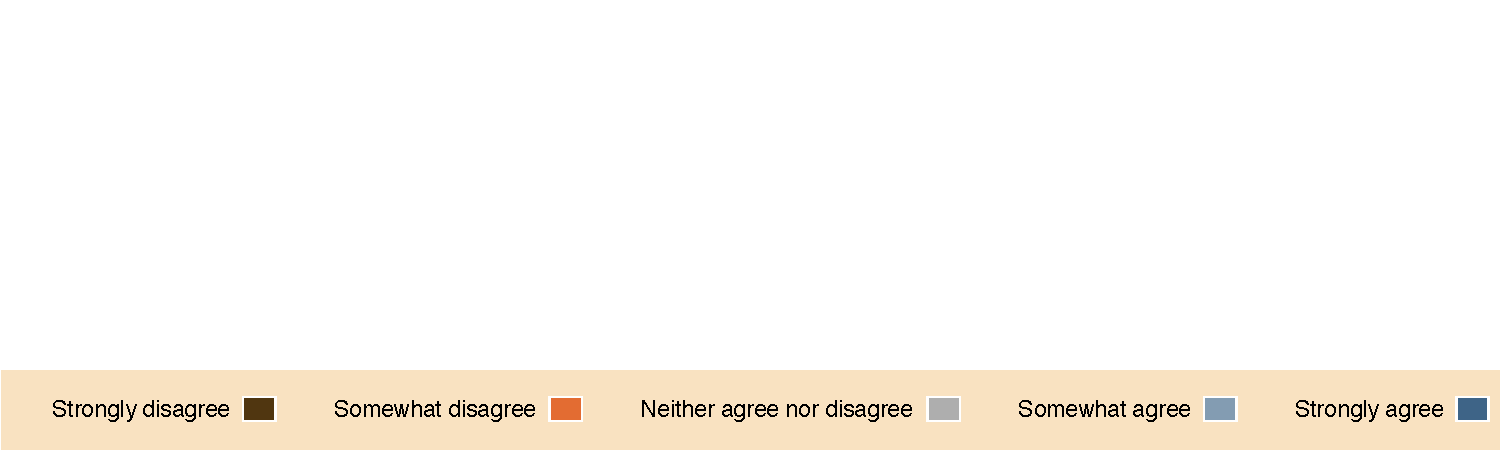
\includegraphics[trim={6mm 0 0 0},clip,width=14.5cm]{fig/legend5col.pdf}
\end{figbox}

\pagebreak 
\subsubsection*{Actions and Priorities}
All actions proposed by the School of Computer Science and Information Technology (CSIT) are presented as follows:

\newtcbtheorem{TEMPaction}{\textsf{ACTION 2.2.1:   Recruitment and Unconscious Bias Training for Research Positions}}{%
        theorem name,%
        separator sign={ },
        borderline west={3pt}{0pt}{RoyalBlue},
        colback=titlebglight!30!white,
        colframe=titlebglight!30!white,
        coltitle=titlebgdark,
        sharp corners,
        left=2mm,
        top=2mm,
        bottom=1mm,
        right=1mm,
        enhanced,
        arc=0pt,
        outer arc=0pt,
        enhanced,
        fonttitle=\sffamily\bfseries\footnotesize,
        fontupper=\sffamily,
        boxrule=0mm,   
        after skip=20pt plus 2pt
    }%
    {TEMPaction}
    
\begin{TEMPaction}{}{}
\actrecruitmenttraining
\hfill{
    \hypersetup{hidelinks}
    \hyperlink{c7}{\gotoactionsymbol{}}
}
\end{TEMPaction}

Actions are numbered in the same way as figures and tables, explained above. The action number is followed by an action title, which is indexed in the List of Actions on Page~\pageref{listofactions}.



The \gotoactionsymbol{} icon is a hyperlink that provides quick access to the Actions table in Section~3. To go back to where the action is introduced, a hyperlink is provided in the Actions table.

On occasion, reference is made to Actions proposed by the university in its institutional Athena Swan Bronze Award Action Plan. These are presented as follows:

\begin{UCCaction}{5.1.3}{}\hypertarget{act513}
Establish a promotion pathway to Professor Scale 1, drawing on learnings for gender equality implemented in schemes for promotion to SL (Jan 2019) and Prof Scale 2 (Oct 2019) scheme calls (see Action 5.1.4).
\end{UCCaction}

Priorities as set out in Section 2.5 are presented as follows:

\begin{priority}{5}
Promote a culture of inclusivity and belonging.
\hfill{
    \hypersetup{hidelinks}
    \hyperlink{p5}{\gotoactionsymbol{}}
}
\end{priority}

The \gotoactionsymbol{} icon is a hyperlink that provides quick access to the appropriate part of the Actions table in Section~3, listing all actions relevant to that particular Priority.

\endgroup 

%TC:endignore 